\title{Project 1 Report} % Title, modify to the name of experiment
\author{Yang Hongmeng}% Author, modify to your name
\date{\today}% Date, Modify to the DATE of EXPERIMENT


 \documentclass[12pt]{article}
\usepackage{graphicx}
\usepackage{booktabs}
 \usepackage{makecell}
 \usepackage{float}
 \newcommand{\diff}{\,\mathrm{d}}
\usepackage[margin=1in]{geometry}
\usepackage{fancyhdr}
\pagestyle{fancy}
\usepackage{extarrows}
\usepackage{breqn}
\usepackage[colorlinks,linkcolor=blue]{hyperref}
\newcommand{\N}{\mathbb{N}}
\newcommand{\Z}{\mathbb{Z}}
\newcommand{\trans}{^{\mathrm T}}
\usepackage{amssymb}
\usepackage[table]{xcolor}
\usepackage{bm}
\usepackage{array}
\usepackage{mathtools}
\usepackage[english]{babel}
\usepackage{natbib}
\usepackage{url}
\usepackage[utf8x]{inputenc}
\usepackage{amsmath}
\usepackage{graphicx}
\graphicspath{{images/}}
\usepackage{parskip}
\usepackage{fancyhdr}
\usepackage{vmargin}
\usepackage[font={bf, footnotesize}, textfont=md]{caption}
\usepackage{amsmath,amsthm,amssymb}


\newenvironment{theorem}[2][Theorem]{\begin{trivlist}
\item[\hskip \labelsep {\bfseries #1}\hskip \labelsep {\bfseries #2.}]}{\end{trivlist}}
\newenvironment{lemma}[2][Lemma]{\begin{trivlist}
\item[\hskip \labelsep {\bfseries #1}\hskip \labelsep {\bfseries #2.}]}{\end{trivlist}}
\newenvironment{exercise}[2][Exercise]{\begin{trivlist}
\item[\hskip \labelsep {\bfseries #1}\hskip \labelsep {\bfseries #2.}]}{\end{trivlist}}
\newenvironment{reflection}[2][Reflection]{\begin{trivlist}
\item[\hskip \labelsep {\bfseries #1}\hskip \labelsep {\bfseries #2.}]}{\end{trivlist}}
\newenvironment{proposition}[2][Proposition]{\begin{trivlist}
\item[\hskip \labelsep {\bfseries #1}\hskip \labelsep {\bfseries #2.}]}{\end{trivlist}}
\newenvironment{corollary}[2][Corollary]{\begin{trivlist}
\item[\hskip \labelsep {\bfseries #1}\hskip \labelsep {\bfseries #2.}]}{\end{trivlist}}
\DeclareMathOperator{\tr}{tr}
\DeclareMathOperator{\rank}{rank}
\DeclareMathOperator{\Span}{span}
\DeclareMathOperator{\row}{row}
\DeclareMathOperator{\col}{col}
\DeclareMathOperator{\range}{range}
\DeclarePairedDelimiterX{\inp}[2]{\langle}{\rangle}{#1, #2}
\DeclareMathOperator{\Proj}{Proj}
\DeclareMathOperator{\trace}{trace}
\newcommand{\Her}{^{\mathrm H}}
\DeclareMathOperator{\diag}{diag}
\makeatletter 
    \newcommand\fcaption{\def\@captype{table}\caption}
\makeatother
\setmarginsrb{3 cm}{2.5 cm}{3 cm}{2.5 cm}{1 cm}{1.5 cm}{1 cm}{1.5 cm}


\makeatletter
\let\thetitle\@title
\let\theauthor\@author
\let\thedate\@date
\makeatother

\pagestyle{fancy}
\fancyhf{}
\rhead{\theauthor}
\lhead{\thetitle}
\cfoot{\thepage}

\begin{document}

\begin{titlepage}
    \centering
    \vspace*{0.5 cm}
    
\includegraphics[scale = 0.75,width=6cm]{CUHK}\\[1.0 cm]   % University Logo
    \textsc{\large The Chinese University of Hong Kong, Shenzhen}\\[2.0 cm] 
    \textsc{\Large CSC4005}\\[0.5 cm] 
    \textsc{\large Parallel Programming}\\[0.5 cm]               % Course Name
    \rule{\linewidth}{0.2 mm} \\[0.4 cm]
    { \huge \bfseries \thetitle}\\
    \rule{\linewidth}{0.2 mm} \\[1.5 cm]
    
    \begin{minipage}{0.4\textwidth}
        \begin{flushleft} \large
            \emph{Author:}\\
            \theauthor
            \end{flushleft}
    \end{minipage}~
    \begin{minipage}{0.4\textwidth}
            \begin{flushleft} \large
            \emph{Student Number:} \\
             119010378  % Modify to your student number
        \end{flushleft}
    \end{minipage}\\[2 cm]
    {\large \thedate}\\[2 cm]
 
    \vfill
    
\end{titlepage}
\tableofcontents
\pagebreak
\rmfamily

\newpage
\section{Introduction}

In this programming project, I implemented odd-even transportation sort algorithm in two methods: parallel execution and sequential execution. Parallel execution method of this algorithm cones from sequential one and parallel computing method was implemented by Message Passing Interface(MPI) method.

Message Passing Interface(MPI) is a standardized and portable messaging-passing standard designed to function on parallel computing architectures. Parallel computing is a type of computation in which many calculations or processes are carried out simultaneously. Large problems can often be divided into smaller ones, which can then be solved at the same time.

Odd-even transportation sort algorithm is a kind of sorting algorithm whose main method is comparing and shifting neighboring elements one by one until all of elements are sorted. At this time, there is no element shifting which is a signal of stop the loop. This algorithm has O($n^{2}$) time complexity when it is executed sequentially.

The purpose of this programming project is letting us learn the basic parallel computing model and trying to analyze the difference between utilizing sequential implementation and parallel computation. Exploring the relationship between sequential method and parallel method of the same algorithm is also vital in this project.

The detailed implementation methods and explanation are shown below.
\section{Material and Method}

In this section, I will introduce how I implement the odd-even transportation algorithm in two ways and how I test my program.

The most common way to implement odd-even transportation sorting algorithm with parallel computing is to implement a sequential one. 

\subsection{Sequential computation method}

\subsubsection{Theoretical Model}

When it comes to implementing a sequential computation method of odd-even transportation algorithm, the first step is to get unsorted input array. In this project, the first step has already been done by the template, and the unsorted input array was stored in the int array named “elements”.

The second step is to sort the data. According to the sorting logic of odd-even algorithm, the odd index elements in the array need to compare with the even index elements before them, which means elements with odd index and greater than 1 should compare them with the element before them. If the odd index elements are smaller than the elements before them, they need to change their position in order to let smaller elements with relatively smaller index. However, if any one of element changes their position in array, the array has not been sorted. Therefore, the algorithm can use whether there is any swap in the array to check whether the array has been sorted, which can be set to a signal of stop the algorithm.

Odd step is followed by even step, and both step has same logic. The only difference is even step using elements with even index which is greater than 2 to compare with the elements with odd index before them. At the same time, the sorted signal can also be changed in the even step. Only when both of even step and odd step do not change any elements’ position, the array is sorted.

The last step is copy sorted array to a new array and wait for output the sorted array to the output file.

\subsubsection{Detailed implementation}

First, get input array to the array named “elements”. This part uses for loop to copy input elements one by one. Therefore, the time complexity here is O(n).

~\\
\centerline {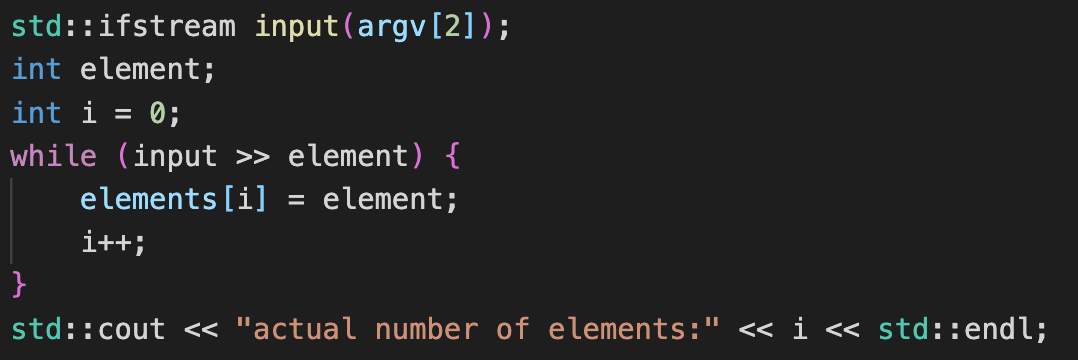
\includegraphics[scale = 1, width=10cm]{input}}
\centerline{\textbf {Figure 1: Get input unsorted array}}

Second, the algorithm will sort the input array. The boolean type variable “sorted” is used to check whether the array has already been sorted. The default value is set to false. 

Next step is using while loop to sort the array step by step until “sorted” with value of true. When the algorithm gets into the while loop, first set the “sorted” value to true. If there is no change in elements’ position, variable “sorted” would also not change its value. Then the while loop will stop. 

However, after setting variable “sorted” value to true, the algorithm will get into the main part of odd-even sorting algorithm. Odd step and even step use for loop to compare elements one by one. If there is any two elements need to change their positions, variable “sorted” will change value to false. It means there is still some elements not in their final positions.

~\\
\centerline {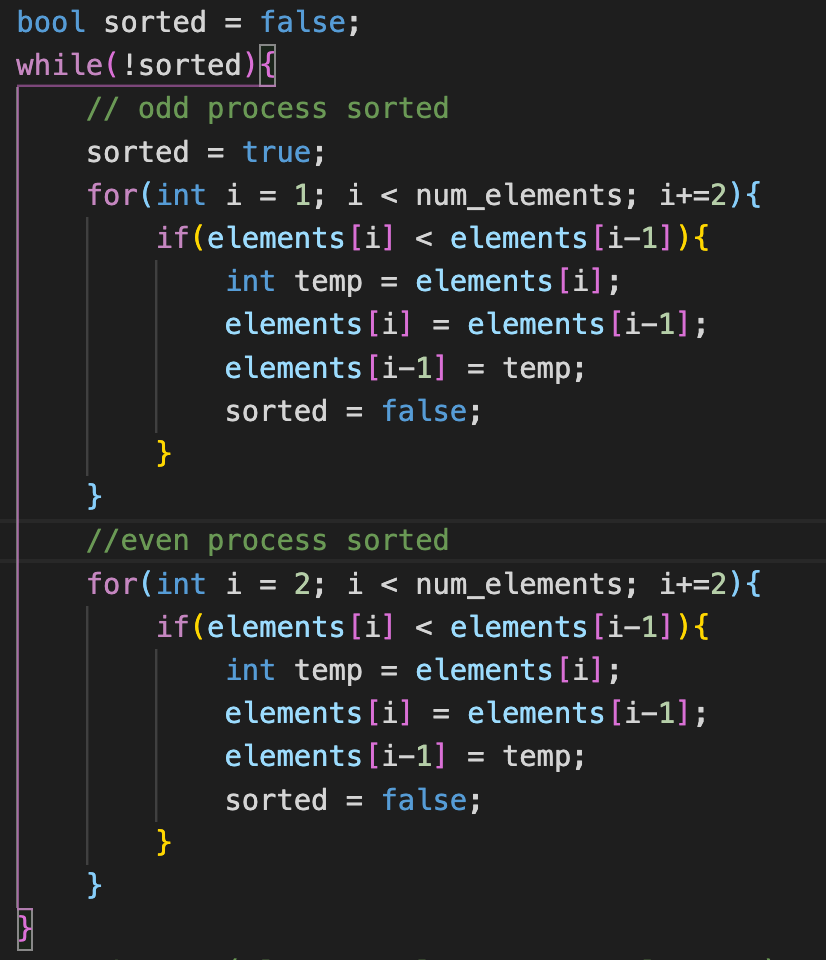
\includegraphics[scale = 1, width=10cm]{seq_imp}}
\centerline{\textbf {Figure 2: Sequential implementation odd-even algorithm sorting part}}

Finally, put all elements in array “elements” to array “sorted\_elements”. Then algorithm stops.

~\\
\centerline {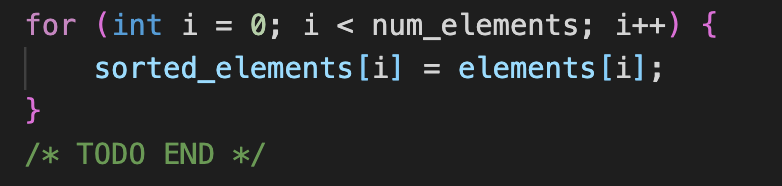
\includegraphics[scale = 1, width=10cm]{seq_final}}
\centerline{\textbf {Figure 3: Final step of sequential implementation}}

\subsection{Parallel computation method}

\subsubsection{Theoretical Model}

After implementing the sequential version of odd-even sorting algorithm, we can change it to parallel version. Nevertheless, there are some problems need to be solved. First, how to evenly distribute elements to each process? Second, how to compare the boundary elements with neighboring processes? Third, is it necessary comparing boundary elements each time? Fourth, how to check whether the local array and total array are both sorted? Finally, how to gather all the elements back?

First, how to evenly distribute elements to each process? We know both elements number and process number are randomly chosen in this project. Therefore, elements may not evenly distribute in each process. However, in order to use “MPI\_Scatter()” function to send elements to each process, we need to make sure that each process gets same number elements. 

The solution of this problem is that we can first check whether elements number can be divisible process number. If it can be divisible, we can use “MPI\_scatter()” function directly. However, if it cannot be divisible, we should add some elements back to the end to make it divisible by process number. We can use elements number mod process number to get the remainder. Then add (process number - remainder) number of elements back to the end of array. Another question which comes from this process is that we need to make sure elements we add to this array will not affect the sorting of original array. At the same time, we know input elements are all integer. Therefore, we just need to add maximum number of integer back to the end and do not put it to the final result.

Second, how to compare the boundary elements with neighboring processes? This problem is one of the most essential and difficult part of parallel programming because we need to be careful to avoid the formation of deadlock. Therefore, I choose to let latter process send first data to previous one and former one blocking receives data. Then the previous process compares its last element with the data received from latter process and send the lager one back to latter process. 

In order to avoid deadlock, I utilize “MPI\_Sendrecv()” function in the latter process and separate blocking receive and send function in former process. At the same time, in order to make sure latter process can put the receive data back to original place, I use same pointer to indicate the location. Finally, in the former process, first step is receiving data sent from latter process. Then do the comparison process and send lager number back.

Third, is it necessary comparing boundary elements each time? It depends on the elements in each process is even number or odd number, and it also depends on the process is odd process or even process. For example, if each process has even number elements, then they need to comparing boundary elements in even processes. On the contrary, if each process has odd number elements, they need to do boundary comparison in odd processes

Fourth, how to check whether the local array and total array are both sorted? In the sequential implementation, we can use whether there is any position change in array to indicate when the algorithm should stop. However, in parallel implementation, we should make sure that all processes do not change any elements position including in-process comparison and elements comparison between two process. Therefore, I used two individual signal to check, one is used to check local array is sorted or not, another is used to gather all local signals and check whether all local arrays are sorted.

The last problem is how to gather all the elements back? I used MPI\_gather() function to gather all local sorted array to the original copied array. Finally, copy the copied array to the final output array named “sorted\_elements”

\subsubsection{Detailed implementation}

In this section, I will introduce the most important part of parallel computing implementation of this project with screenshot of my code. At the same time, the difference between sequential and parallel implementation will also show here.

\textbf{First step: process input data}

The first difference is getting input. In order to protect the input data and save executing time, I let only process0 do the read input execution (showed in Figure 4).

~\\
\centerline {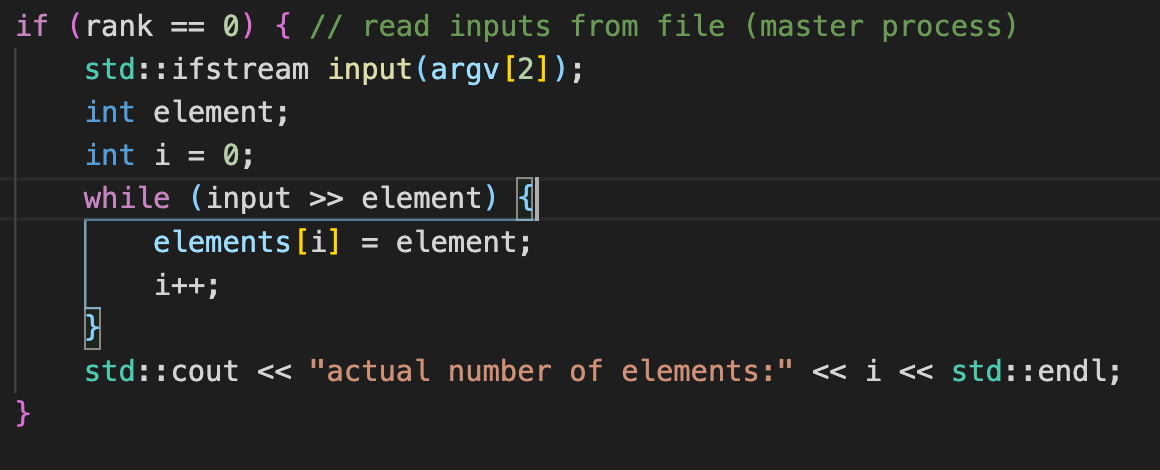
\includegraphics[scale = 1, width=10cm]{para_input1}}
\centerline{\textbf {Figure 4: Final step of sequential implementation}}

Compared with sequential implementation, parallel implementation need to separate input data to each individual process which is also done by process0. Figure 5 shows the main process of processing data and send data to different processes. 

The first step is copy the input array to a predefined vector because vector can extend its size by utilizing “push\_back()” function, which is helpful for make elements number is divisible by process number.

The second step is to calculate the remainder of element number mod process number. If the remainder is 0 which means elements number is divisible by process number, then the vector do not need to add extra elements. Otherwise, the vector should add some elements to make elements number is divisible by process number.

The last step is to calculate the size of elements that each process will receive. Because the algorithm has already processed data before, it must be an integer.

~\\
\centerline {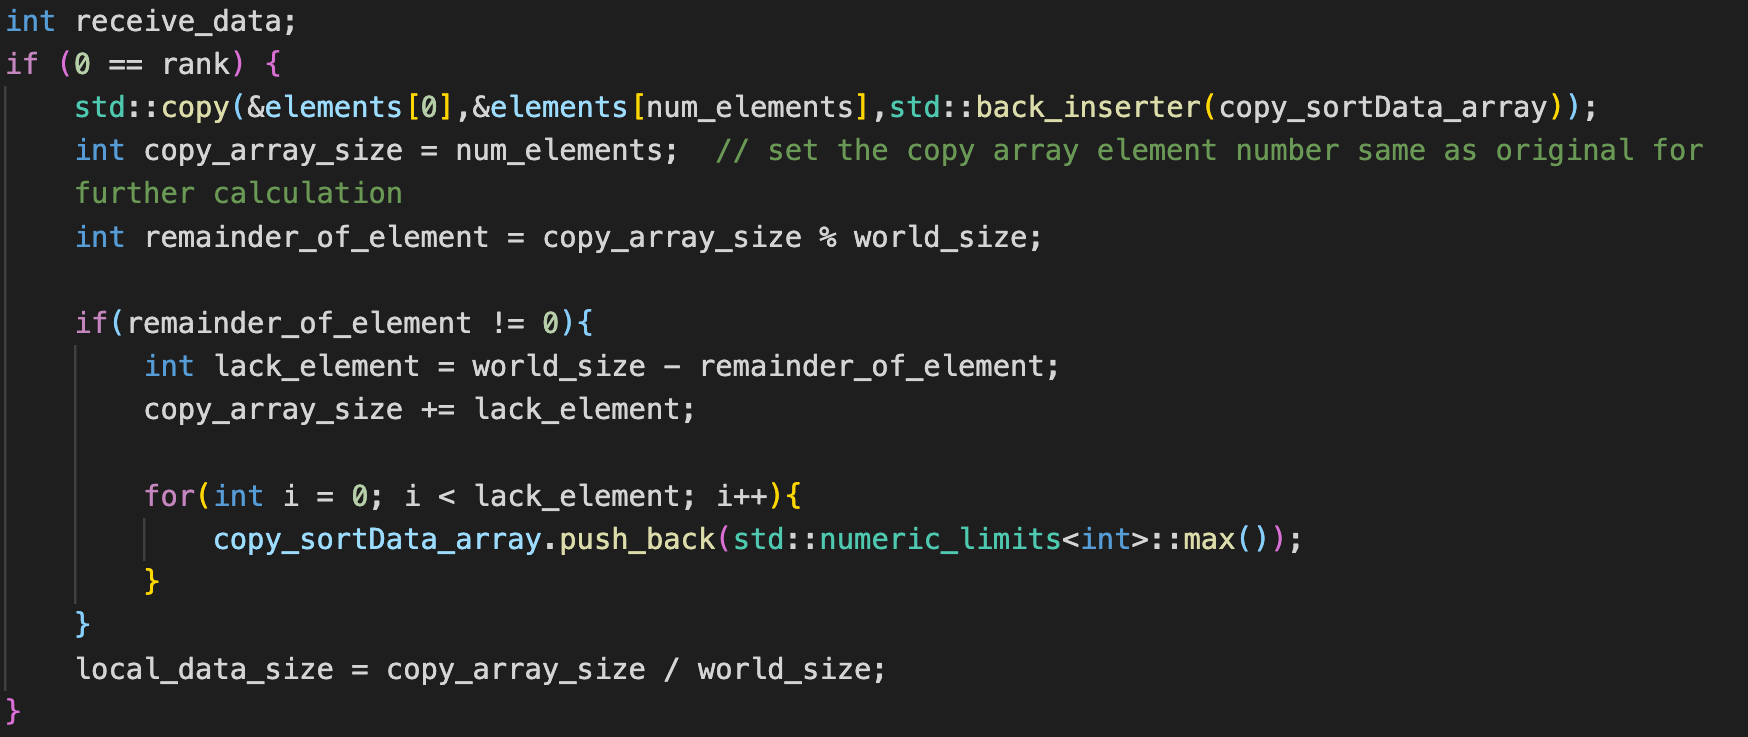
\includegraphics[scale = 1, width=14cm]{para_input2}}
\centerline{\textbf {Figure 5: Final step of sequential implementation}}

The last step of getting input part is send unsorted data to each process. In order to let each process can receive data, all process need to create a local vector. Before each process creating local vector, process0 should send local vector size to each process. I use “MPI\_Bcast()” function to send local vector size. And each process create local vector. Finally, process0 uses “MPI\_Scatter()” function separate the processed vector in process0 to each process.

~\\
\centerline {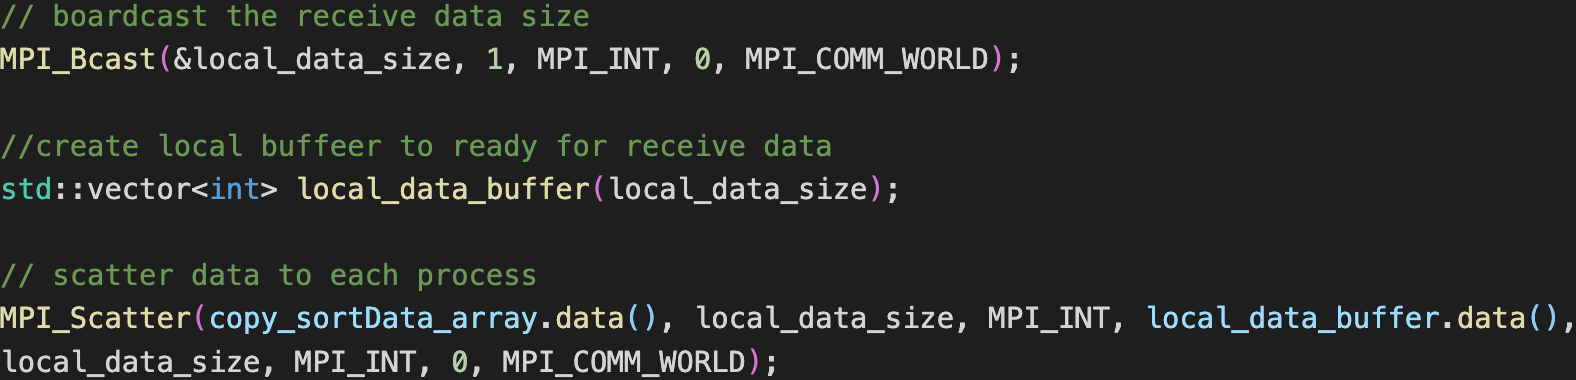
\includegraphics[scale = 1, width=14cm]{para_input3}}
\centerline{\textbf {Figure 6: Final step of sequential implementation}}

~\\
\textbf{Second step: executing sorting algorithm}

First I create two boolean variable “local\_sorted” and “total\_sorted” to indicate whether local vector is sorted and whether all local vectors are sorted. “total\_sorted” can get from logic and all “local\_sorted”. If all “local\_sorted” are true, it means total vector is sorted and the algorithm can gather data back. “local\_sorted” is like variable “sorted” in sequential implementation. It would be set to true when the process get into sorting while loop.

In parallel implementation, each process will also do odd process comparison and even process comparison locally. The difference between parallel implementation and sequential implementation is that parallel implementation need to do boundary comparison between neighboring processes after both odd process and even process.

Figure 7 shows boundary comparison in odd step. Boundary comparison can be divided into three parts. First, if there is total odd number processes, the last process do not need to participate into boundary comparison. Second, if process number is odd number, it needs to send its first element to previous process to do the comparison. Odd number processes also need to receive data from previous process and put it to the first position of array. Finally, the other even number processes first receive the data from latter process and compare its last element with received data. If its last elements is greater than received data, then it will change its last data to received data and send its original last data to latter process. Otherwise, it will not change received data element and just send it back.

~\\
\centerline {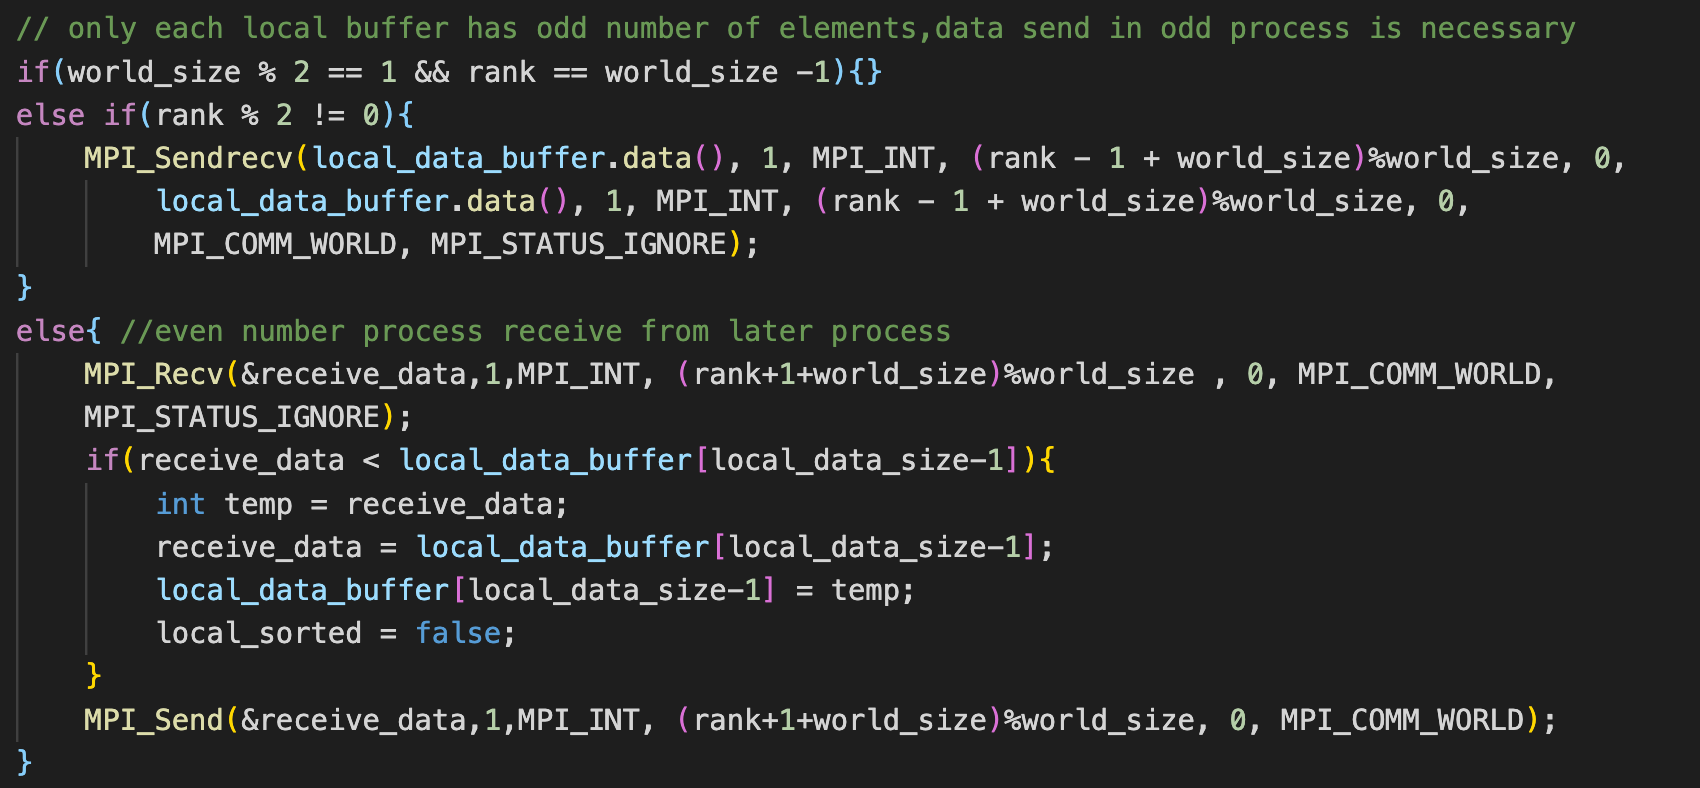
\includegraphics[scale = 1, width=14cm]{para_bo}}
\centerline{\textbf {Figure 7: Boundary comparison implementation in odd step}}

There are two differences between odd step boundary comparison and even step comparison. First, in even step boundary comparison, process0 do not need to do any execution and if total process number is an even number, then the last process also do not need to do any process. Second, in even step, even number processes send their last element to previous process and odd number processes receive data and do comparison execution. The even step boundary comparison is shown below.

~\\
\centerline {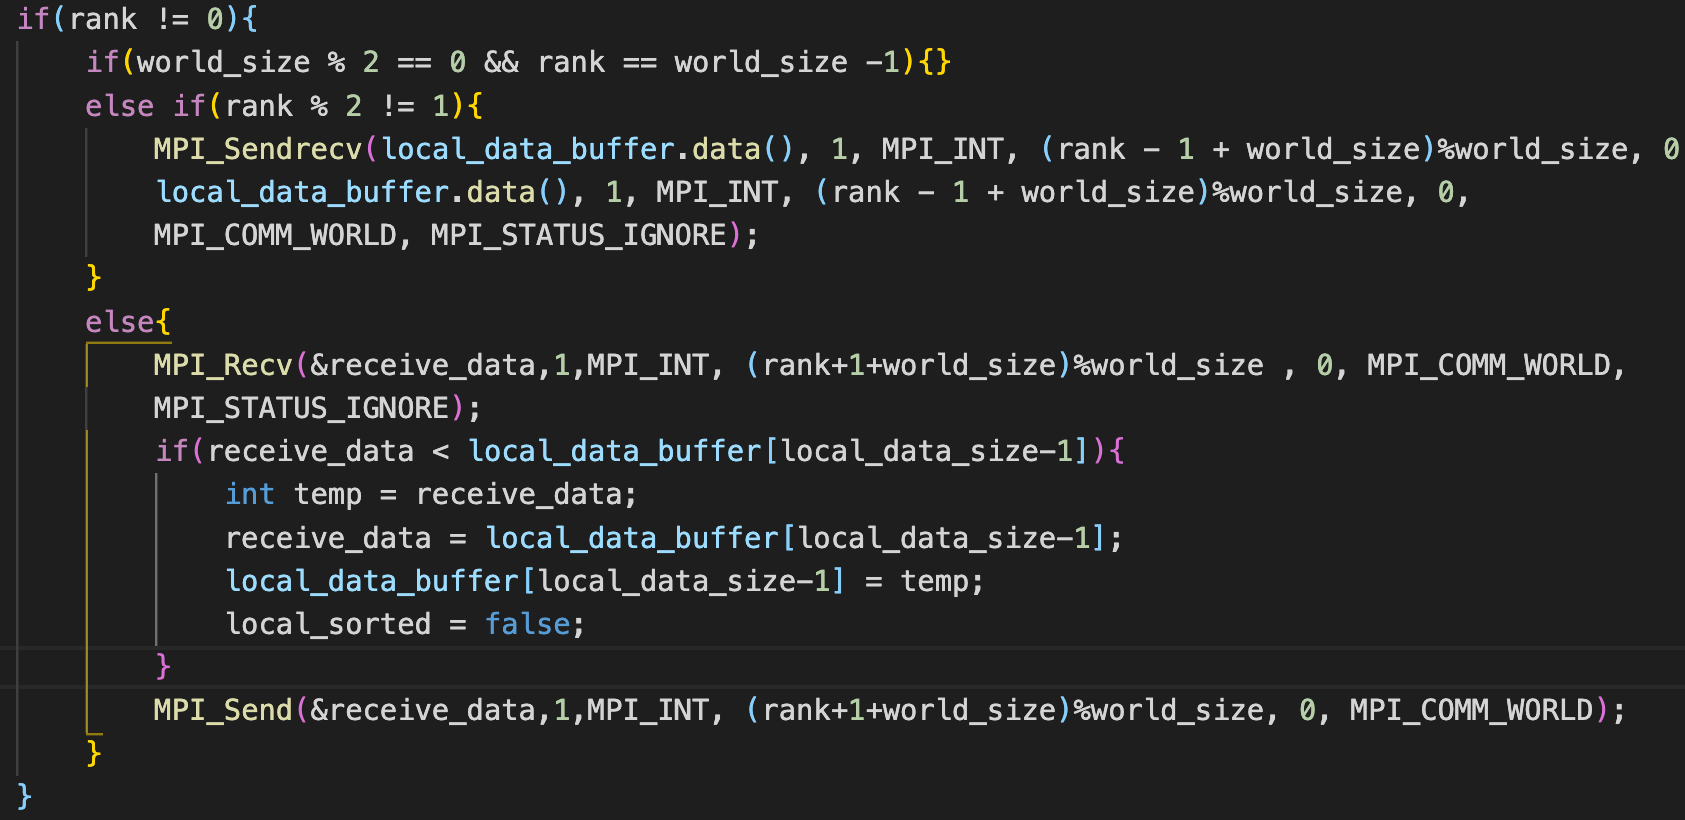
\includegraphics[scale = 1, width=14cm]{para_bo2}}
\centerline{\textbf {Figure 8: Boundary comparison implementation in even step}}

The last step is checking whether the array has been sorted. This can be indicated by variable “total\_sorted”. In order to get value of “total\_sorted”, I use function “MPI\_Reduce()” and using MPI\_LAND as MPI operation during MPI\_Reduce. After getting the value of “total\_sorted” broadcast its value to all process which can stop all process.

~\\
\centerline {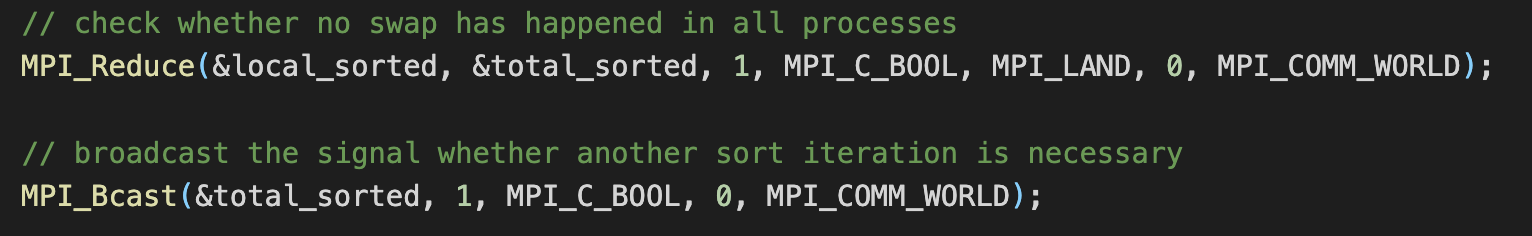
\includegraphics[scale = 1, width=14cm]{para_bo3}}
\centerline{\textbf {Figure 9: Stop signal checking}}

\textbf{Third step: Gathering elements back}

The final step of parallel implementation is gather all elements back and copy sorted array to output array “sorted\_elements”

~\\
\centerline {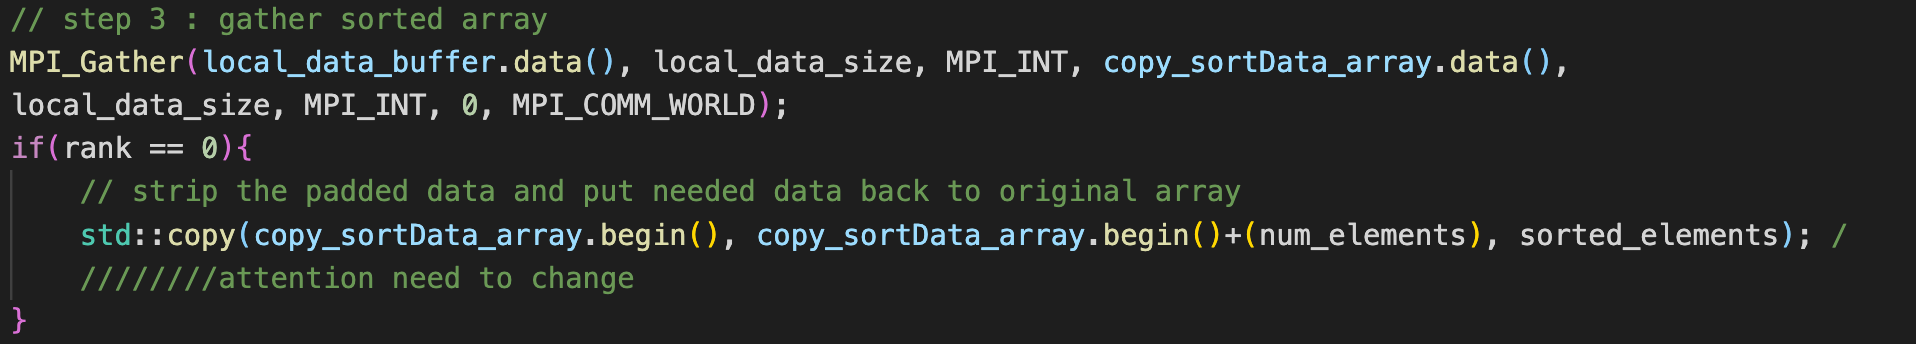
\includegraphics[scale = 1, width=14cm]{para_bo4}}
\centerline{\textbf {Figure 10: Gather elements}}

\subsection{Compile and test both codes}

In this section, I will introduce how to compile and test my code. 

In order to compile and execute my code, you can directly run file “sequential.sh” and “parallel.sh” by utilizing command “sh sequential.sh” or “sh parallel.sh”. These two file will help you compile two of my code directly and execute them. If you want to change the test dataset, you can change the range of variable “ele\_num” in “parallel.sh”. You can also change the core number of execution by changing the number of variable of “core” in  file “parallel.sh”. 

You need to pay attention that, only “parallel.sh” can generate test data for you, and in order to test the difference between sequential execution and parallel execution, test dataset should be the same. Therefore, you can execute “parallel.sh” first and execute “sequential.sh” to compare the performance of two implementation. You can also generate dataset by yourself to only test sequential execution performance. 

When you execute these two file, they will create two folder to store the result. For parallel execution, you can check result in folder “report\_result”. In this folder you can choose to see different core number execution by choosing the folder name with the core number. At the same time, these two file will also help you check whether the data has been sorted. The checking result will show at the end of the result file. All of output files are from terminal output.

\section{Result Analysis:}

\subsection{Theoretical analysis}
\subsubsection{Time complexity}

\textbf{Sequential implementation:}

Assuming there are n input elements. For both odd step and even step, the algorithm needs to do ($\frac{n}{2}$) comparison. Therefore, in each step, the time complexity is O(n). 

Now we first calculate the time complexity of best case, which means the input array is sorted. The algorithm just needs to do one odd step and one even step to know that the input array is sorted. Therefore, the time complexity of best case is O(n).

Another one is the worst case, which means the input array is sorted by descending order. The first element needs n time shifting to get back to the end of array. According to previous analysis, we know the time complexity of each odd-even operation is O(n). Therefore, the time complexity of worst case is O($n^2$).

\textbf{Parallel implementation:}

For parallel execution, each process can get $\frac{n}{p}$ elements. And time complexity of each odd-even process is O($\frac{n}{p}$) or O(n).

For worst case, the first element would use n times shifting from the first element of first process to the last element of last process. Therefore, the time complexity of the parallel execution would be O($\frac{n^2}{p}$) or O($n^2$).

For the best case, the algorithm just need O($\frac{n}{p}$) or O(n) time to know the array has been sorted. Therefore, the time complexity of the best case is O($\frac{n}{p}$) or O(n).

\subsubsection{Speedup}


According to the equation of speedup, we know S(n)=$\frac{t_{s}}{t_{p}}$. Speedup is equal to the execution time of sequential execution ($t_{s}$) divided by execution time of parallel execution ($t_{p}$).

\subsubsection{Efficiency}

According to the equation of efficiency we know E=$\frac{S(n)}{n}$. Efficiency is equal to the speedup of n processes divided by process number. 

\subsection{Result analysis}

\subsubsection{Execution time}

Figure below shows the execution time of sequential execution of odd-even algorithm. According to our analysis above, we can know if the input number enlarge to twice of original input, execution would be four times of original execution time. The curve showed on the figure is the execution time of input size of 10000 times square of input elements number divide 10000. We can conclude from the figure that the experiment results are near the line. Therefore, it can be an evidence of time complexity of sequential execution is O($n^2$).

~\\
\centerline {\includegraphics[scale = 1, width=13cm]{seq_data}}
\centerline{\textbf {Figure 11: Sequential execution result}}

The following two figures show the execution result of parallel execution. We can learn from the first figure is that when the dataset is small, lager process number may decrease the performance. When dataset is 40000, it is most obvious. If we set process number to 40000, the execution time would be larger than previous one, which means the performance of the code decreases.

~\\
\centerline {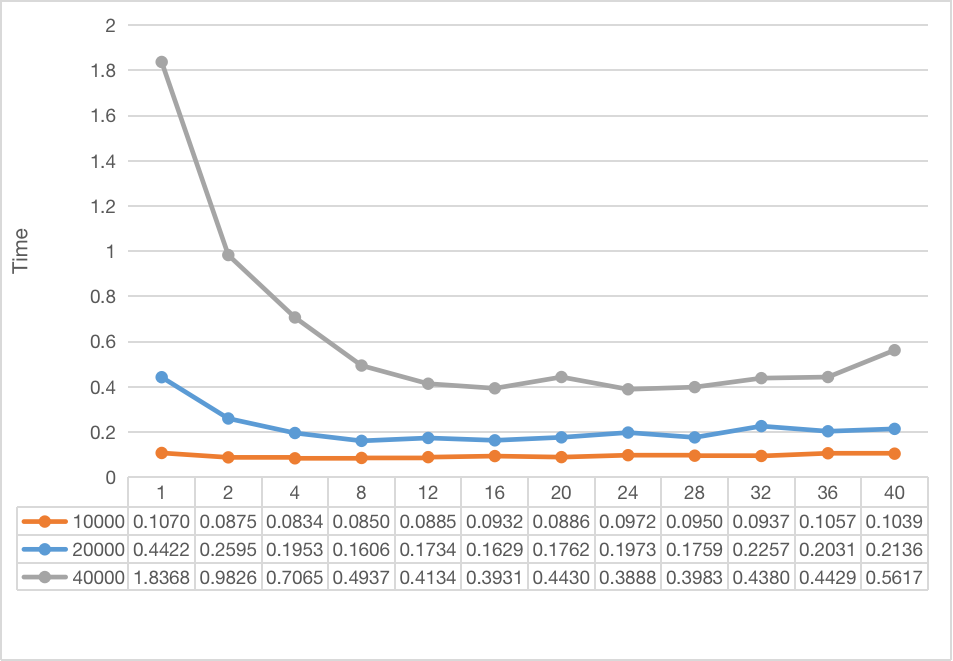
\includegraphics[scale = 1, width=12cm]{small_data}}
\centerline{\textbf {Figure 12: Parallel execution result with small input number}}

When it comes to the large number input, it is obvious that with the increase of process number, the execution drop dramatically. Therefore, we can conclude that if input is large enough, the more process number, the less execution time.

~\\
\centerline {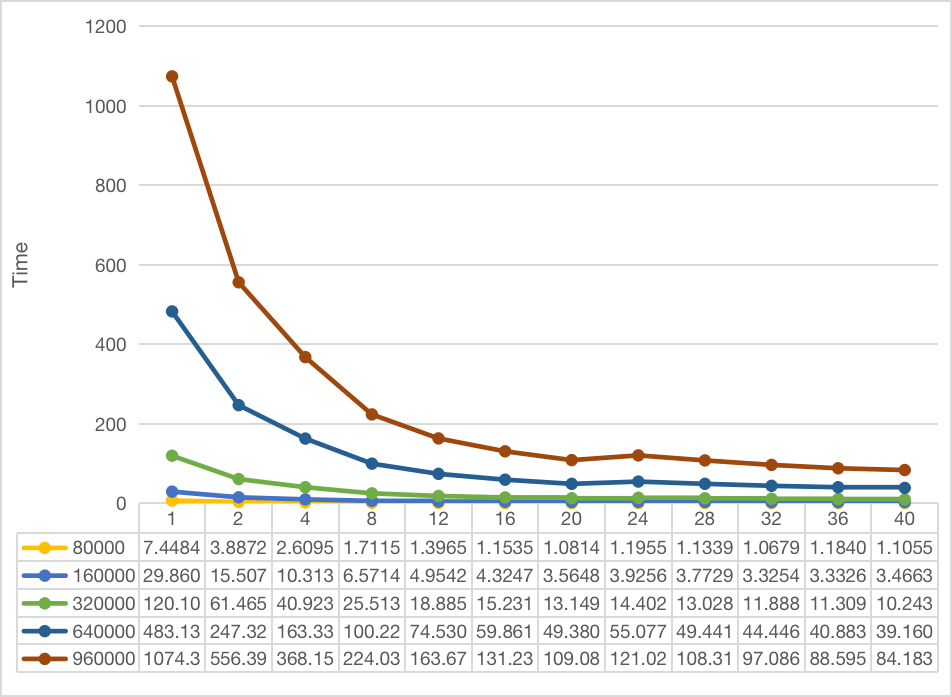
\includegraphics[scale = 1, width=14cm]{large_data}}
\centerline{\textbf {Figure 13: Parallel execution result with large input number}}

\subsubsection{Speedup}

The following figure shows the speedup of my test result. From this figure we can know with the increase of process number, the speedup increase. However, we can also learn that the increasing rate of speedup is not a constant. The possible reason is that this algorithm cannot be finished totally by only parallel executing. There are some communication between each process, and there are also sequential execution in this algorithm. 

At the same time, we can also conclude that after process number larger than some certain the increase of speedup is not obvious. We can observe the speedup line of 36 processes and 40 processes. It is hard to see difference between these two lines, although they are not completely the same.

~\\
\centerline {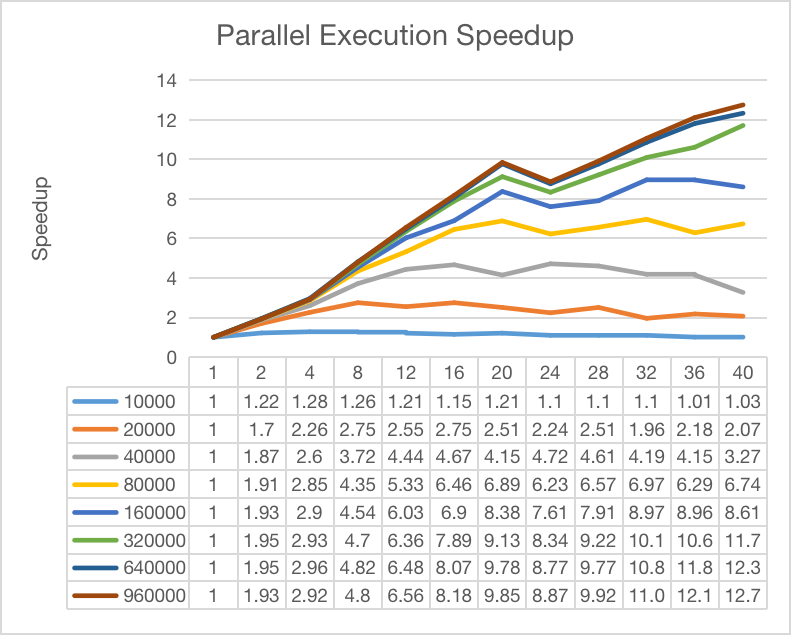
\includegraphics[scale = 1, width=14cm]{speedup}}
\centerline{\textbf {Figure 14: Speedup of parallel execution result}}

\subsubsection{Efficiency}

After getting the speedup, I use speedup divide their corresponding process number to get efficiency of the experiments. And the results are showed in below figure. The efficiency shows descending tendency with the increase of process number. With the increase of input elements number, the efficiency increases.

~\\
\centerline {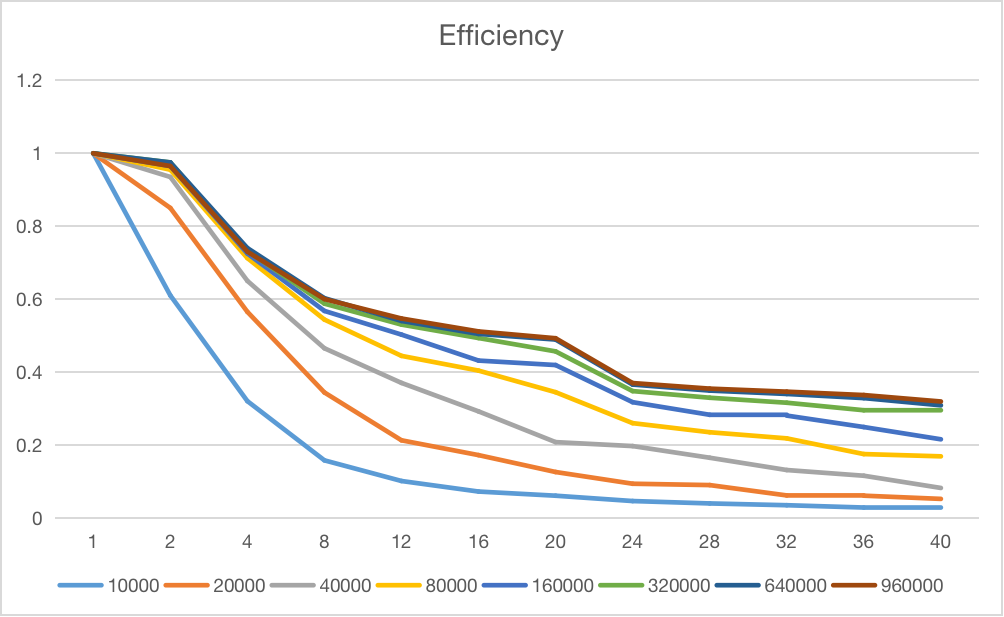
\includegraphics[scale = 1, width=14cm]{eff}}
\centerline{\textbf {Figure 15: Efficiency of parallel execution result}}

\section{Conclusion}

In this project, I learn the basic parallel computing model and utilizing MPI to implement a parallel execution code. At the same time, I also tried to debug a parallel execution code. During implementing the program, I learn how processes communicate with each other and how one process send and receive data from other processes. 

After finishing the test experiment and analyzing result, I found that more process number or more core used in parallel computing does not means better performance. After the number of process larger than some certain number, the performance will decrease. 

Finally, after calculating the efficiency, I found that parallel computing can use less execution time, but it need more resource and the efficiency shows that parallel computing is less efficient than sequential execution according my implementation.

\section{Appendix}

In this section, I will show the demo input and output of my parallel implementation code. There are 20 random input number and three processes number result are the same. Therefore, I just put one screenshot here. I choose three parallel implementation output: process number 1, 8 and 20. Because they represent three special case: all elements in one process, number of elements in each process are different and the case of each process only has one element.

~\\
\centerline {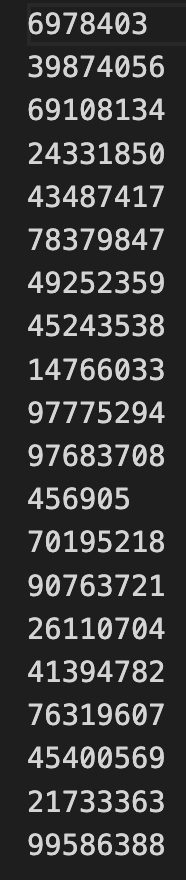
\includegraphics[scale = 1, width=3.5cm]{para_in}}
\centerline{\textbf {Figure 16: Demo input with 20 elements}}
~\\
\centerline {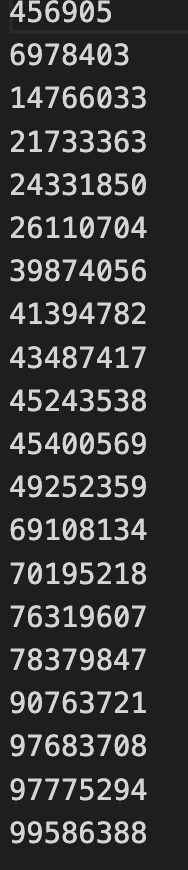
\includegraphics[scale = 1, width=4cm]{para_out}}
\centerline{\textbf {Figure 17: Demo output with 20 elements}}
~\\
\centerline {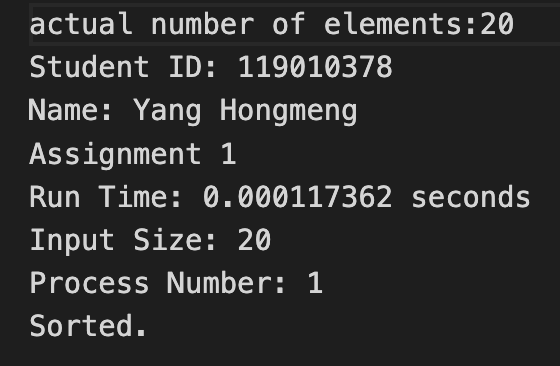
\includegraphics[scale = 1, width=14cm]{para_1}}
\centerline{\textbf {Figure 18: Parallel code output with 1 process}}

~\\
\centerline {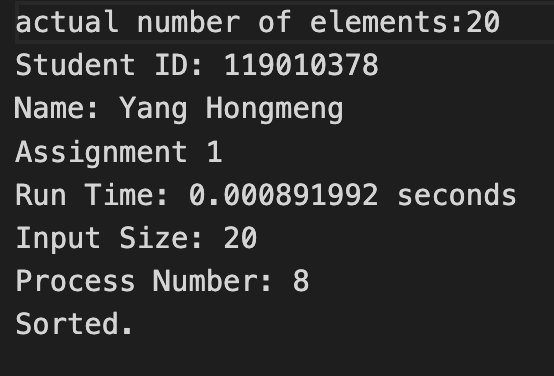
\includegraphics[scale = 1, width=14cm]{para_8}}
\centerline{\textbf {Figure 19: Parallel code output with 8 processes}}

~\\
\centerline {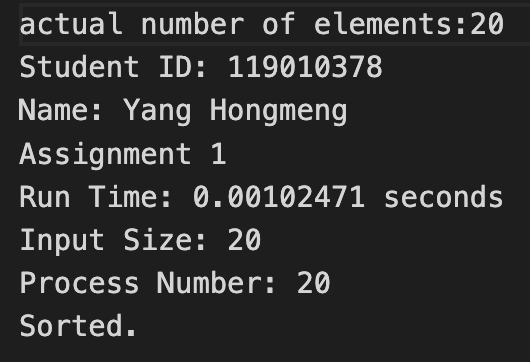
\includegraphics[scale = 1, width=14cm]{para_20}}
\centerline{\textbf {Figure 20: Parallel code output with 20 processes}}

\end{document}
